\begin{frame}{Decoding Strategies: Greedy vs Sampling}
  \begin{itemize}
    \item[\textcolor{red}{$\blacktriangleright$}] \textbf{Greedy/Beam Search:} Generates less surprising, often boring responses.
    \begin{itemize}
      \item Not desirable for open-ended tasks like dialog and story-telling.
    \end{itemize}
    \item[\textcolor{red}{$\blacktriangleright$}] \textbf{Sampling:} Used for more diverse and creative outputs.
  \end{itemize}
  \begin{center}
    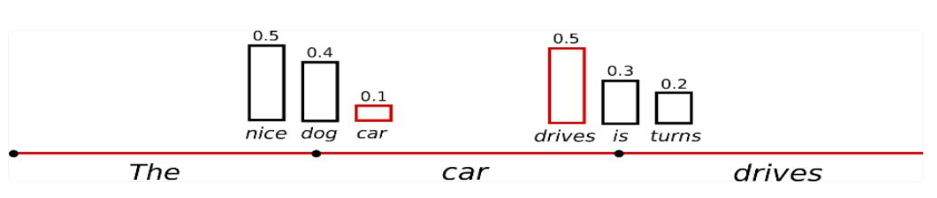
\includegraphics[width=0.85\linewidth]{images/prompting-rag/prompting_decoding_token_probabilities.png}
  \end{center}
\end{frame}

\begin{frame}{Key Sampling Parameters: Temperature and Top $p$}
  \begin{itemize}
    \item[\textcolor{red}{$\blacktriangleright$}] \textbf{Temperature}
    \begin{itemize}
      \item Controls sharpness of the next-token distribution.
      \item Typically between 0 and 2 (higher values give more random outputs).
      \item Lower temperature $\rightarrow$ sharper distribution $\rightarrow$ more repetitive generations.
    \end{itemize}
    \item[\textcolor{red}{$\blacktriangleright$}] \textbf{Top $p$ (Nucleus Sampling)}
    \begin{itemize}
      \item Value between 0 to 1.
      \item Select the smallest set of tokens whose total likelihood exceeds $p$; redistribute the probabilities.
      \item Smaller $p$ leads to more repetitive generations.
    \end{itemize}
  \end{itemize}
  {\scriptsize
    \textbf{Source:} \url{https://huggingface.co/blog/how-to-generate}
  }
\end{frame}
